\documentclass[a4paper]{article}
\usepackage[margin=1.5cm]{geometry}
\usepackage{mathpazo}
\usepackage{hyperref}
\hypersetup{colorlinks=true,linkcolor=blue,citecolor=blue,filecolor=blue,urlcolor=blue}
\usepackage{nicefrac}
\usepackage{amsmath}
\usepackage{amssymb}
\usepackage{graphicx}
% allow to add python code snippets easily
\usepackage{listings}
\lstset{language=Python, basicstyle=\ttfamily\small, showstringspaces=false, numbers=left, numberstyle=\tiny, numbersep=5pt, breaklines=true, frame=lines, backgroundcolor=\color{gray!10}, breakatwhitespace=true, escapeinside={(*@}{@*)}}
% enable syntax highlighting for python with listings
\usepackage{color}

% define macro for upright d in integrals
\newcommand{\dd}{\mathrm{d}}


% create macro 'fixme' in red text
\usepackage{xcolor}
\newcommand{\fixme}[1]{\textcolor{red}{#1}}

\begin{document}
\section{Big bang thermodynamics}
\subsection{Moments of the distribution function}
The universe becomes hotter and denser as we go to earlier times. This leads to a heat bath in which many processes can occur in equilibrium. As the heat bath decreases in energy with the expansion of the Universe, these processes will freeze out and stop. We will now lay some foundations for understanding the physics behind this. In general, one express the statistical properties of a large number of particles in terms of their distribution function, which gives their density in six-dimensional phase space (3 positions $\times$ 3 momentum coordinates). The distribution function $f(\mathbf{x},\mathbf{p},t)$ is then a positive function of these six coordinates and time. The number density, energy density and pressure which are functions only of the position can then be given by integrating out the velocity dimensions (marginalising over them). Since we assume that the Universe is homogeneous, they will be identical at every point in space and it suffices to consider them as functions of time only. Since the Universe is also isotropic, there will also be no directional dependence in the momenta $\mathbf{p}$, so that we can simply work with the modulus of the momentum $p$. We then have
\begin{align}
\text{particle number density} && n(t) & =  4\pi \int f(p,t) \;p^2 {\rm d}p \\
\text{energy density} && c^2\rho(t) & = 4\pi\int E(p) \;f(p,t) p^2 {\rm d}p \\
\text{pressure} && P(t) & =  4\pi \int \frac{p^2 c^2}{3E(p)} f(p,t) \;p^2 {\rm d}p.
\end{align}
Energy and momentum of particles are related through the relativistic momentum equation as $E^2 = p^2c^2+m^2c^4$. The term in the expression for the pressure comes from the usual definition of the kinetic pressure of a gas $P=\frac{1}{3}n\left<p v\right>$ and the relativistic momentum which gives $v = p c^2/E$.


\begin{table}[h]
  \centering
  \begin{tabular}{l|c|c}
  \hline
  \textbf{Particle} & \textbf{Spin} & \textbf{Degeneracy factor} \\
  \hline
  \hline
  Electron & \nicefrac{1}{2} & 2 \\
  \hline
  Photon & 1 & 2 \\
  \hline
  Quark & \nicefrac{1}{2} & 6 \\
  \hline
  Neutrino & \nicefrac{1}{2} & 1 \\
  \hline
  \hline
  Massive scalar & 0 & 1 \\
  Massless scalar & 0 & \fixme{?} \\
  \hline
  Massive vector & 1 & 3 \\
  Massless vector & 1 & 2 \\
  \hline
  Massive tensor & 2 & 5 \\
  Massless tensor & 2 & \fixme{?} \\
  \hline
  \hline
  \end{tabular}
  \caption{\label{tab:degeneracy} Spin and degeneracy factors for some particles.}
  \end{table}

\subsection{Fermi-Dirac and Bose-Einstein Statistics}
If the particles are in a thermodynamic equilibrium state, they will follow either a Fermi-Dirac or a Bose-Einstein distribution function, depending on the species of the particles. These distributions are
\begin{equation}
f(p,t) =   \frac{g}{(2\pi \hbar)^3}\left[\exp\left(\frac{E(p)-\mu}{kT(t)}\right)\pm 1\right]^{-1},
\end{equation}
where the '+' version holds for fermions (spin-1/2) particles and the '-' version for bosons (integer spin). The pre-factor $g$ is a spin degeneracy factor and depends on the number of possible spin states for the particle type (cf.~\autoref{tab:degeneracy}), and $\mu$ is the chemical potential. The chemical potential is a measure of the energy required to add a particle to the system. For a system in equilibrium, the chemical potential is constant in space and time. 

\subsection{Critical density and density parameters}
The critical density today is defined as
\begin{align}
\rho_{\rm crit} & = \frac{3H_0^2}{8\pi G} = 1.88\times 10^{-29} \;h^2\; \frac{\rm g}{{\rm cm}^3} = 2.78\times 10^{11}\;h^2\;\frac{M_\odot}{{\rm Mpc}^3} 
\intertext{while in terms of the associated energy density one has}
c^2\rho_{\rm crit} &= \frac{3H_0^2c^2}{8\pi G}  = 1.05\times 10^{-5}\;h^2\;\frac{\rm erg}{{\rm cm}^3}.
\end{align}

\subsection{Important limits}
\paragraph{Non-relativistic limit.} The particles are non-relativistic if $m^2c^4\gg p^2 c^2$. In this case one can expand the energy in the distribution function as
\begin{align}
  E(p) = \sqrt{m^2c^4+p^2c^2} = mc^2 + \frac{p^2}{2m} + \mathcal{O}\left(\frac{p^4}{m^3c^2}\right)
\end{align}
 and the distribution function becomes
\begin{align}
f(p,t) & = \frac{g}{(2\pi \hbar)^3}\left[\exp\left(\frac{mc^2+p^2/2m-\mu}{k_{\rm B}T(t)}\right)\pm 1\right]^{-1} \;.
\end{align}
In the non-relativistic case thermal energy must be much less than the rest mass energy $k_{\rm B}T \ll mc^2$ since $k_{\rm B}T$ is $\bar{p}^2/2m$ in terms of a mean $\bar p$.  This implies that $\exp(E(p)/{k_{\rm B}T})\gg 1$ and the distribution function becomes identical for bosons and fermions and is given by the Maxwell-Boltzmann distribution
\begin{align}
f(p,t) & \simeq \frac{g}{(2\pi \hbar)^3}\exp\left[-\frac{mc^2+p^2/2m-\mu}{k_{\rm B}T(t)}\right] =  \frac{g}{(2\pi \hbar)^3}\exp\left[\frac{\mu-mc^2}{k_{\rm B}T(t)}\right]\exp\left[\frac{p^2}{2mk_{\rm B}T(t)}\right]\;.
\end{align}
It is then easy to carry out the integrals above and one finds
\begin{equation}
n(T) = g\left(\frac{mk_{\rm B}T}{2\pi}\right)^{3/2}\exp\left[\frac{\mu-mc^2}{k_{\rm B}T}\right],\quad\rho(t)= mn(t),\quad P(t) = nk_{\rm B}T.
\end{equation}
which implies \fixme{this is not right:}
\begin{align}
  \Omega(T) = \frac{\rho(T)}{\rho_{\rm crit}} = \frac{m}{\rho_{\rm crit}}\left(\frac{mk_{\rm B}T}{2\pi}\right)^{3/2}\exp\left[\frac{\mu-mc^2}{k_{\rm B}T}\right].
\end{align}

\paragraph{Ultrarelativistic limit.} The other limit one can easily calculate is for the ultrarelativistic ($k_{\rm B}T\gg mc^2$) limit where 
\begin{align}
E(p) &= pc, & f(p,t) &= \frac{g}{(2\pi \hbar)^3}\left[\exp\left(\frac{pc-\mu}{k_{\rm B}T(t)}\right)\pm 1\right]^{-1}
\end{align}
We shall further assume the non-degenerate ($\mu\ll k_{\rm B}T$) case. In this limit one finds for \textbf{fermions}
\begin{align}
n(T) &= g\frac{3\,\zeta(3)}{4\pi^2}\frac{k_{\rm B}^3T^3}{c^3\hbar^3}, & \rho(T)& =g\frac{7\pi^2}{240}\frac{k_{\rm B}^4 T^4}{c^5\hbar^3}, & P(T) &= \rho(T)/3
\end{align}
so that
\begin{align}
\Omega(T) &= \frac{\rho(T)}{\rho_{\rm crit}} = g\frac{7\pi^3}{90}\frac{G k_{\rm B}^4 T^4}{c^5\hbar^3 H_0^2} \simeq 2.40840498\times10^{-5} \;g\;\left(\frac{h}{0.67}\right)^{-2}\;\left(\frac{T}{2.725 {\rm K}}\right)^4.
\end{align}
and for \textbf{bosons}
\begin{align}
n(T) &= g\frac{ \zeta (3)\;k_{\rm B}^3 T^3}{ \pi ^2 c^5 \hbar^3},& \rho(T)&=g\frac{\pi^2}{30}\frac{k_{\rm B}^4T^4}{c^3\hbar^3}, & P(T) &= \rho(T)/3,
\end{align}
so that
\begin{align}
\Omega(T) &= \frac{\rho(T)}{\rho_{\rm crit}} = g\frac{4\pi^3  }{45  }\frac{G k_{\rm B}^4T^4}{c^5\hbar^3H_0^2}\simeq 2.75246283\times10^{-5} \;g\;\left(\frac{h}{0.67}\right)^{-2}\;\left(\frac{T}{2.725 {\rm K}}\right)^4.
\end{align}
In particular, note that 
\begin{align}
  \rho_\text{fermion} = \frac{7}{8}\rho_\text{boson}.
\end{align}
\paragraph{The effective number of relativistic species.} The energy density in relativistic species can be written as
\begin{align}
  \rho_\text{rel} = \frac{\pi^2}{30}\;\frac{k_{\rm B}^4}{c^3\hbar^3}\;g_\text{eff}(T)\; T^4,
\end{align}
The effective number of relativistic degrees of freedom is given by
\begin{align}
  g_\text{eff}(T) = \sum_{i\in\text{bosons}}g_i + \frac{7}{8}\sum_{i\in\text{fermions}}g_i =g_\text{bosons} + \frac{7}{8} g_\text{fermions}.
\end{align}
\paragraph{The relativistic degrees of freedom of the standard model.} Let us calculate the effective number of relativistic degrees of freedom for the standard model of particle physics. The list of bosons with their respective degrees of freedom before, and after, electroweak symmetry breaking is
\begin{enumerate}
  \item The photon: $g_\gamma=2$ (massless spin-1) 
  \item The $W^\pm$ and $Z$ bosons: $3\times2\text{(massless spin-1)}=6$ (before) and $3\times3\text{(massive spin-1)}=9$ (after).
  \item The 8 gluons: $8\times 2\text{(massless spin-1)}=16$.
  \item The Higgs boson: $4$ (before) and $1$ (after).
\end{enumerate}
The list of fermions with their respective degrees of freedom is
\begin{enumerate}
  \item The massive leptons: $e^\pm$, $\mu^\pm$, $\tau^\pm$: $3\text{(families)}\times2\text{(anti)}\times2\text{(massive spin-1/2)}=12$.
  \item The massless leptons: $\nu_{e,\mu\tau}$, $\bar{\nu}_{e,\mu,\tau}$: $3\text{(families)}\times 2\text{(anti)}\times 1\text{(massless spin-\nicefrac{1}{2})}=6$.
  \item The six quarks and antiquarks: $6\text{(types)}\times2\text{(anti)}\times2\text{(massive spin-\nicefrac{1}{2})}\times3\text{(color)}=72$.
\end{enumerate}
Therefore the total number of relativistic degrees of freedom is
\begin{align}
  g_\text{eff}(T>100 \text{GeV}) = \left(2+6+16+4\right)\;+\; \frac{7}{8}\left(12+6+72\right) = 106.75.
\end{align}

\subsection{Neutrino temperature}
The ratio of the temperature of relic photons $T_\gamma$ and neutrinos $T_\nu$ is given by
\begin{align}
  T_\nu = \left(\frac{4}{11}\right)^{1/3}T_\gamma.
\end{align}
The neutrino temperature is therefore $T_\nu\approx1.95$K. The neutrino temperature is determined by the temperature of the photons at the time of neutrino decoupling. 


\subsection{Beyond standard model physics: massive neutrinos}
Massive neutrinos are fermions with mass $m_\nu$ and spin $1/2$. The number of spin degrees of freedom is $g=2$ (instead of 1 in the massless case) and the chemical potential is zero. We shall assume three generations of massive neutrinos with distinct mass eigenstates $m_{\nu_i}$. The shall be produced in thermal equilibrium as ultrarelativistic species, and are subsequently redshifted. Their energy density is then given by
\begin{align}
  \Omega_\nu(T) &= g \frac{4G }{3\pi \hbar^3 H_0^2} \sum_{i=1}^3 \int_0^\infty \; \frac{p^2\sqrt{m_{\nu_i}^2c^4+p^2c^2}  }{\exp\left[\frac{pc}{k_{\rm B}T_\nu a^{-1}}\right]+1}\;{\rm d}p\\
  &= g \frac{4G }{3\pi \hbar^3 H_0^2} \sum_{i=1}^3 \int_0^\infty \; \frac{\frac{p^2}{m_{\nu_i}^2c^2}m_{\nu_i}^3c^4\sqrt{1+\frac{p^2c^2}{m_{\nu_i}^2c^4}}  }{\exp\left[\frac{pc}{k_{\rm B}T_\nu a^{-1}}\right]+1}\;{\rm d}p
  \intertext{Let now $\beta_i:=\frac{m_{\nu_i} c^2}{k_{\rm B}T_\nu}$ and $y_i:=a \frac{p}{m_{\nu_i} c}$ so that $\dd y_i = a \frac{\dd p}{m_{\nu_i} c}$. Then}
  \Omega_\nu(T) &= a^{-3}\;g \frac{4Gc^5 }{3\pi \hbar^3 H_0^2} \sum_{i=1}^3 m_{\nu_i}^4\;\int_0^\infty \; \frac{ y_i^2\sqrt{1+\frac{y_i^2}{a^2}}  }{\exp\left[\beta_i y_i\right]+1}\;{\rm d}y_i\\
  &= a^{-3}\;g \frac{4Gc }{3\pi \hbar^3 H_0^2} \sum_{i=1}^3 m_{\nu_i}^4\;\int_0^\infty \; \frac{ x^2\sqrt{1+x^2/a^2}  }{\exp\left[\beta_i x\right]+1}\;{\rm d}x
\end{align}
So that finally,
\begin{align}  
  \boxed{\Omega_\nu(T) = a^{-3}h^{-2}  \sum_{i=1}^3 g_i \left(\frac{m_{\nu_i}}{6.32264\;\nicefrac{\rm meV}{\rm c^2}}\right)^4\;\int_0^\infty \; \frac{ x^2\sqrt{1+x^2/a^2}  }{\exp\left[\beta_i x\right]+1}\;{\rm d}x}\label{eq:omeganu}
\end{align}

\subsection{Extra radiation and effective number of neutrinos}
The relativistic energy density of the universe is given by the sum of the photon energy density and the neutrino energy density, parameterized through the effective number of relativistic neutrinos $N_\text{eff}$ as
\begin{align}
  \rho_r = \rho_\gamma + \rho_\nu = \rho_\gamma \left(1+\frac{7}{8} \left(\frac{T_\gamma}{T_\nu}\right)^{\nicefrac{1}{3}}\;N_\text{eff}\right) = \rho_\gamma \left(1+\frac{7}{8} \left(\frac{4}{11}\right)^{\nicefrac{4}{3}}\;N_\text{eff}\right).
\end{align}


% show python code snippet that computes Omega_nu(T) for a given T, given the three distinct neutrino masses as input
% \begin{lstlisting}[language=Python]
% import numpy as np
% from scipy.special import kn
% from scipy.constants import c, hbar, k, pi

% def Omega_nu( a, mnu ):
%     """
%     Computes the neutrino density parameter Omega_nu for a given scale factor a and neutrino mass mnu
%     a: scale factor
%     mnu: neutrino mass in eV
%     """
%     T = T_CMB/a
%     k = 8.6173303e-5 # eV/K
%     hbar = 6.58211928e-16 # eV*s
%     H0 = 2.2685455e-18 # 1/s
%     c = 299792458 # m/s
%     Omega_nu = 0.0
%     for i in range(3):
%         Omega_nu += 2*7*pi/960*(mnu[i]/(k*T))**2*kn(2,mnu[i]/(k*T))
%     Omega_nu *= k**4*T**4/c**5/hbar**3/H0**2
%     return Omega_nu
% \end{lstlisting}


\section{Perturbation equations in synchronous gauge following Ma and Bertschinger}
\subsection{Metric perturbations}
\begin{align}
  k^2\eta - \frac{1}{2}\frac{\dot{a}}{a}\dot{h} &= 4\pi G a^2 \delta T^0_{\phantom{0}0}  \\
  k^2\dot{\eta} &= 4\pi G a^2 (\overline{\rho}+\overline{P})\;\theta \\
  \ddot{h} + 2\frac{\dot{a}}{a}\dot{h} - 2k^2\eta &= -8\pi G a^2 \delta T^i_{\phantom{i}i} \\
  \ddot{h} + 6 \ddot{\eta} + 2\frac{\dot{a}}{a}\left(\dot{h}+6\dot{eta}\right) - 2k^2\eta &= -24\pi G a^2 (\overline{\rho}+\overline{P})\;\sigma
\end{align}

\subsection{CDM}
\begin{align}
  \dot{\delta_c} &= - \frac{\dot{h}}{2} \\
  \theta_c = \sigma_c &= 0
\end{align}

\subsection{Baryons}
\begin{align}
  \dot{\delta}_b &= -\theta_b - \frac{\dot{h}}{2} \\
  \dot{\theta}_b &= -\frac{\dot{a}}{a}\theta_b + c_s^2k^2\delta_b + \frac{4\overline{\rho}_\gamma}{3\overline{\rho}_b}a n_e \sigma_T (\theta_\gamma-\theta_b)\\
  c_s^2 &= \frac{k_B T_b}{\mu}\left(1-\frac{1}{3}\frac{\dd \log T_b}{\dd \log a}\right)\\
  \dot{T}_b &= -2\frac{\dot{a}}{a}T_b + \frac{8}{3}\frac{\mu}{m_e}\frac{\overline{\rho}_\gamma}{\overline{\rho}_b} a n_e \sigma_T (T_\gamma-T_b).
\end{align}

\subsection{Photons}
\begin{align}
  \dot{\delta}_\gamma &= -\frac{4}{3}\theta_\gamma - \frac{2}{3}\dot{h} \\
  \dot{\theta}_\gamma &= k^2\left( \frac{1}{4}\delta_\gamma - \sigma_\gamma \right) + a n_e \sigma_T\left(\theta_b-\theta_\gamma\right)\\
 2 \dot{\sigma}_\gamma = \dot{F}_{\gamma}^{(2)} &= \frac{8}{15}\theta_\gamma - \frac{3}{5}k F_{\gamma}^{(3)} + \frac{4}{15} \dot{h} + \frac{8}{5} \dot{\eta} - \frac{9}{5}a n_e \sigma_T \sigma_\gamma + \frac{1}{10}a n_e \sigma_T(G_{\gamma}^{(0)}+G_{\gamma}^{(2)})\\
  \dot{F}_{\gamma}^{(\ell)} &= \frac{k}{2\ell+1}\left[\ell F_{\gamma}^{(\ell-1)}-(\ell+1)F_{\gamma}^{(\ell+1)}\right] - a n_e \sigma_T F_{\gamma}^{(\ell)}\;,&&\text{for $\ell_\text{max}>\ell\ge3$}\\
  \dot{F}_{\gamma}^{(\ell_\text{max})} &\approx k F_{\gamma}^{(\ell_\text{max}-1)} - \frac{\ell_\text{max}+1}{\tau}F_{\gamma}^{(\ell_\text{max})} - a n_e \sigma_T F_{\gamma}^{(\ell_\text{max})} \\
  \dot{G}_{\gamma}^{(\ell)} &= \frac{k}{2\ell+1}\left[\ell G_{\gamma}^{(\ell-1)}-(\ell+1)G_{\gamma}^{(\ell+1)}\right] + \nonumber \\
  &\quad + a n_e \sigma_T \left[-G_{\gamma}^{(\ell)}+\frac{1}{2}\left(F_{\gamma}^{(2)}+F_{\gamma}^{(0)}+G_{\gamma}^{(2)}\right)\left(\delta_{\ell0}+\frac{1}{5}\delta_{\ell2}\right)\right]\;,&&\text{for $\ell_\text{max}>\ell\ge3$} \\
  \dot{G}_{\gamma"}^{(\ell_\text{max})} &\approx k G_{\gamma}^{(\ell_\text{max}-1)} - \frac{\ell_\text{max}+1}{\tau}G_{\gamma}^{(\ell_\text{max})} - a n_e \sigma_T G_{\gamma}^{(\ell_\text{max})}
\end{align}



\subsection{Massless neutrinos}
\begin{align}
  \dot{\delta}_\nu &= -\frac{4}{3}\theta_\nu - \frac{2}{3}\dot{h} \\
  \dot{\theta}_\nu &= k^2\left( \frac{1}{4}\delta_\nu - \sigma_\nu \right) \\ 
  2 \dot{\sigma}_\nu = \dot{F}_{\nu}^{(2)} &= \frac{8}{15}\theta_\nu - \frac{3}{5}k F_{\nu}^{(3)} + \frac{4}{15} \dot{h} + \frac{8}{5} \dot{\eta}\\
  \dot{F}_{\nu}^{(\ell)} &= \frac{k}{2\ell+1}\left[\ell F_{\nu}^{(\ell-1)}-(\ell-1)F_{\nu}^{(\ell+1)}\right] \\
  F_{\nu}^{(\ell_\text{max}+1)} &\approx \frac{(2\ell_\text{max}+1)}{k\tau} F_{\nu}^{(\ell_\text{max})} - F_{\nu}^{(\ell_\text{max}-1)}  
\end{align}

\subsection{Massive neutrinos}
\begin{align}
  \dot{\psi}_0 &= -\frac{qk}{\epsilon}\psi_1 + \frac{1}{6}\dot{h}\frac{\dd \log f_0}{\dd \log q}\;, \\
  \dot{\psi}_1 &= \frac{qk}{3\epsilon}\left(\psi_0 - 2\psi_2\right)\;,\\
  \dot{\psi}_2 &= \frac{qk}{5\epsilon}\left(2\psi_1 - 3\psi_3\right) - \left(\frac{1}{15}\dot{h} + \frac{2}{5}\dot{\eta}\right)\frac{\dd \log f_0}{\dd \log q}\;,\\
  \dot{\psi}_\ell &= \frac{qk}{(2\ell+1)\epsilon}\left(\ell\psi_{\ell-1} - (\ell+1)\psi_{\ell+1}\right)\;,\qquad\text{for $\ell\ge3$}\;,\\
  \psi_{\ell_\text{max}+1} &\approx \frac{(2\ell_\text{max}+1)\epsilon}{qk\tau} \psi_{\ell_\text{max}} - \psi_{\ell_\text{max}-1}\;.
\end{align}
so that the neutrino perturbations are given by
\begin{align}
  \delta\rho_\nu &= \frac{4\pi}{a^4}\int \dd q\;q^2\epsilon f_0(q)\psi_0(q)\;,\\
  \delta P_\nu &= \frac{4\pi}{3a^4}\int \dd q\;\frac{q^4}{\epsilon} f_0(q)\psi_1(q)\;,\\
  (\overline{\rho}_\nu+\overline{P}_\nu)\theta_\nu &= \frac{4\pi k}{a^4}\int \dd q\;q^3 f_0(q)\psi_1(q)\;,\\
  (\overline{\rho}_\nu+\overline{P}_\nu)\sigma_\nu &= \frac{8\pi}{3a^4}\int \dd q\;\frac{q^4}{\epsilon} f_0(q)\psi_2(q)\;.
\end{align}

% \subsection{Photons}
% \begin{align}
  
% \end{align}

\section{Approximations}
\begin{figure}
  \centering
  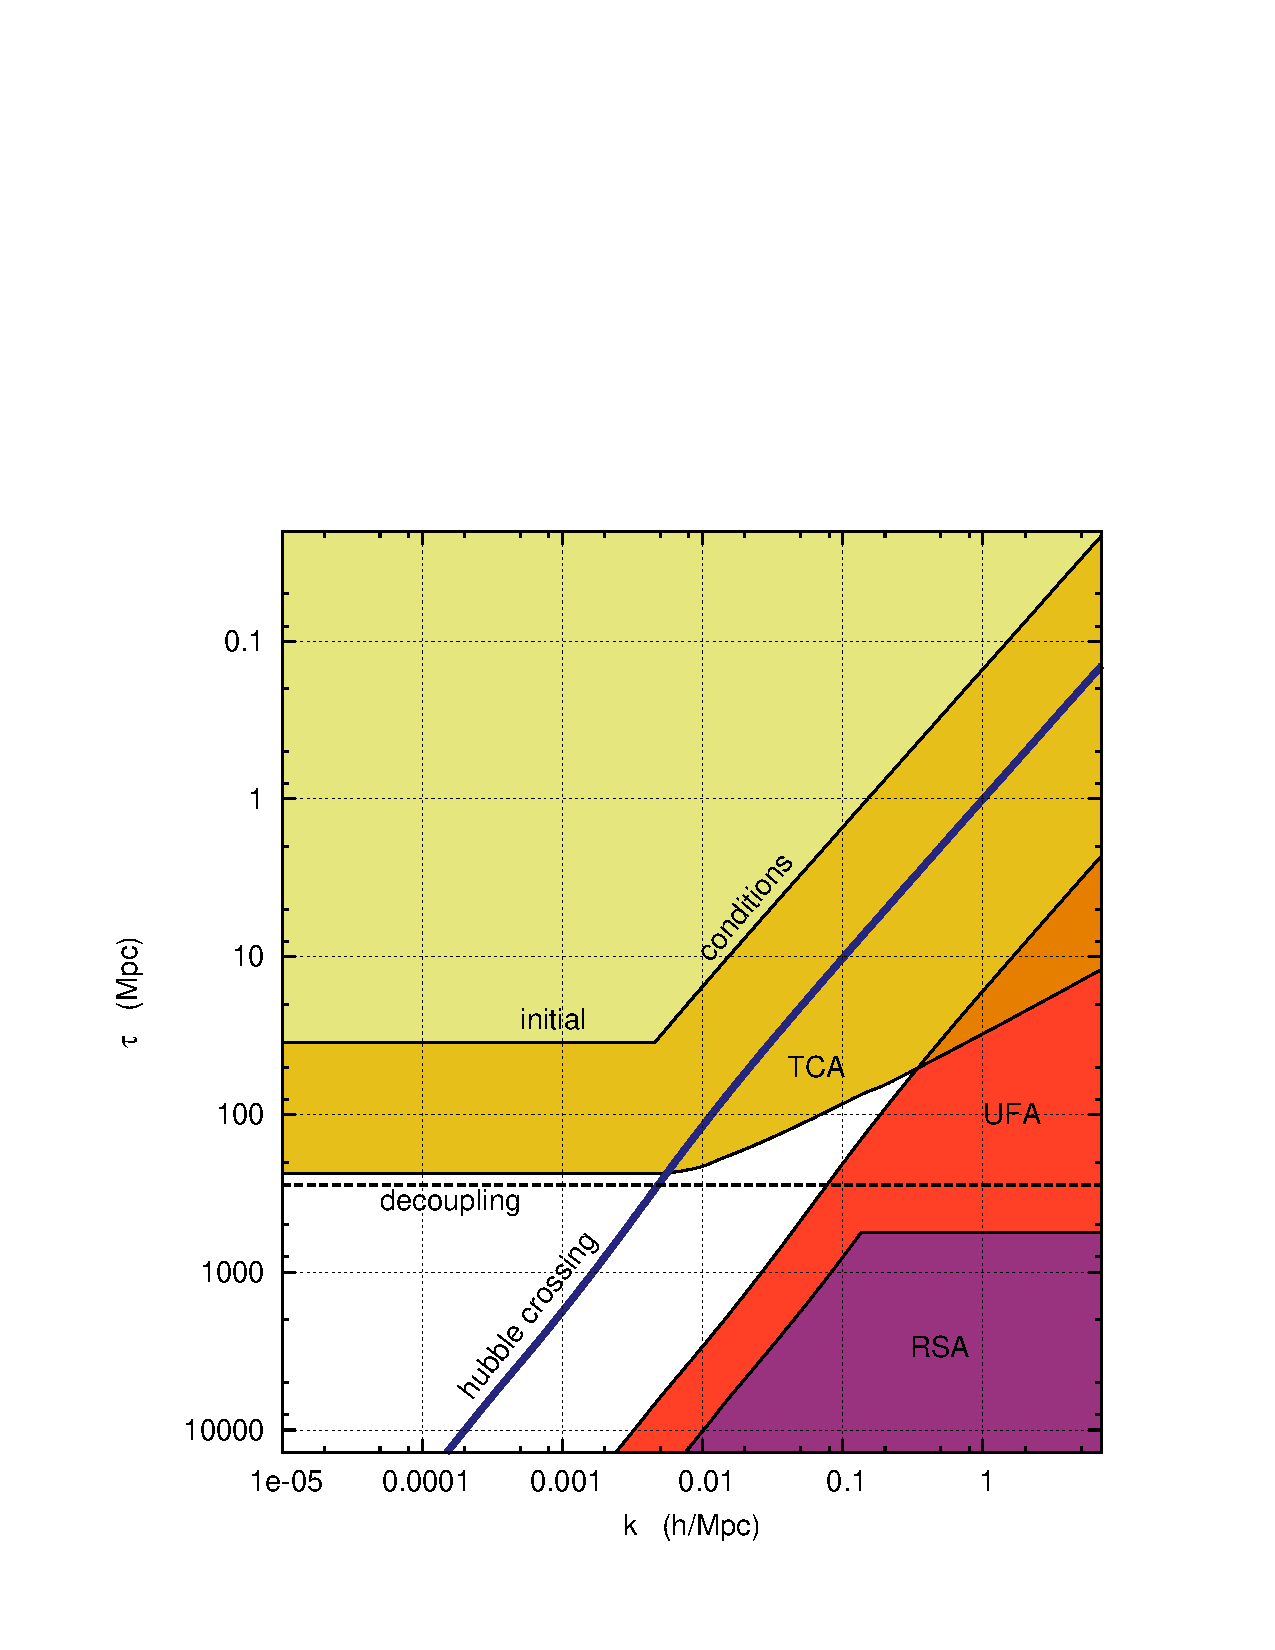
\includegraphics[width=0.5\textwidth]{approx_summary.pdf}
  \caption{Overview over approximations employed in CLASS, cf. BLT11 (CLASS-II)}
  \label{fig:approx_overview}
\end{figure}

The approximations in CLASS, and in which regime they are switched on, can be seen in Figure~\ref{fig:approx_overview}.

\end{document}
